\chapter{設計と実装}
\label{chap:implementation}

\section{構成}

本研究において実装したESP32上で動作するプログラムの実装の構成を示す。

まず、WebAssembly Core Specification\cite{wasm_spec}により規定された仕様を基に、
WebAssemblyインタプリタをライブラリとして実装した(libwasm)。
libwasmは、標準C(C11)により規定された仕様のみを用いて、プラットフォーム非依存な形で実装した。

次に、定数として保持した静的なWebAssemblyバイナリをlibwasmを用いて実行し、
結果を出力するだけの簡単なプログラムを、ESP-IDF\cite{esp_idf}を用いてFreeRTOS上に実装した。

全体の構成を図\ref{fig:esp32_libwasm}に示す。

\begin{figure}[htbp]
  \caption{本実装の構成}
  \label{fig:esp32_libwasm}
  \begin{center}
    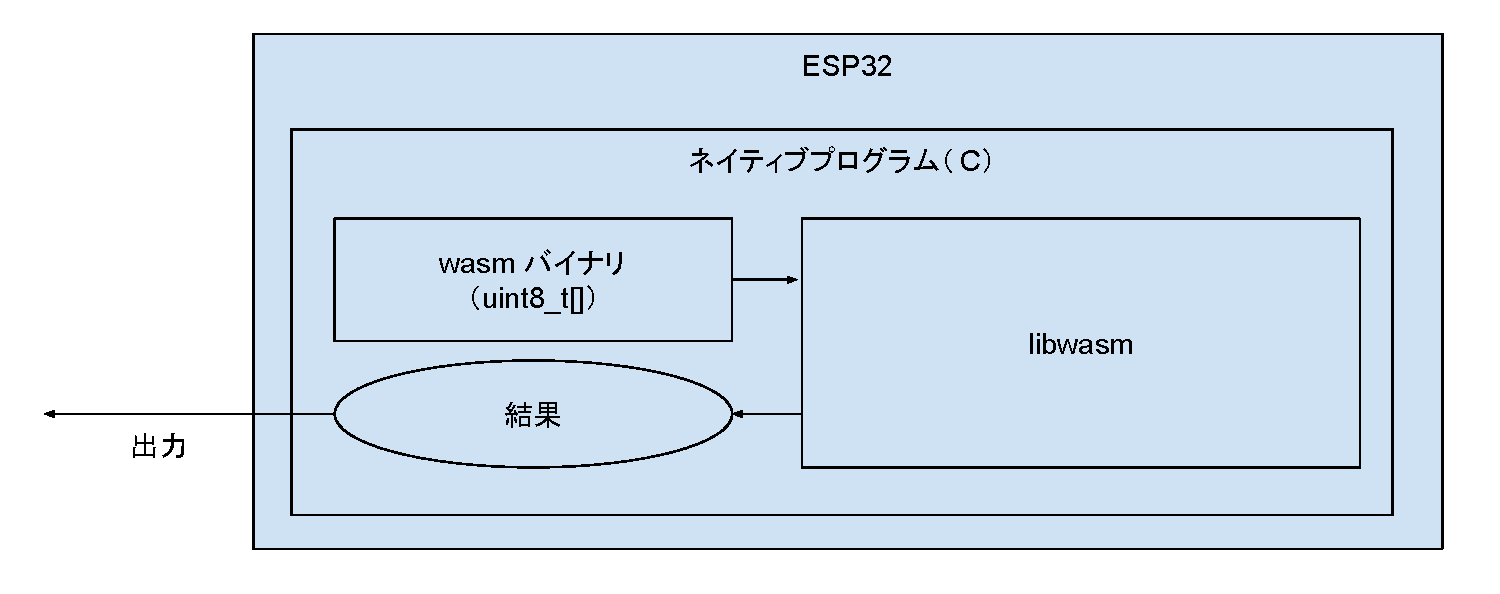
\includegraphics[bb=0 0 800 300,width=12cm]{img/esp32_libwasm.pdf}
  \end{center}
\end{figure}

続いて、libwasmの構成を\ref{fig:libwasm_arch}に示す。

libwasmは、大きく分けてパーサ部と実行部からなる。

パーサは、WebAssemblyバイナリ(バイト列)を受け取ってWebAssemblyモジュール
(\verb|wasm_module_t|)としてデコードする。


\begin{figure}[htbp]
  \caption{libwasmの構成}
  \label{fig:libwasm_arch}
  \begin{center}
    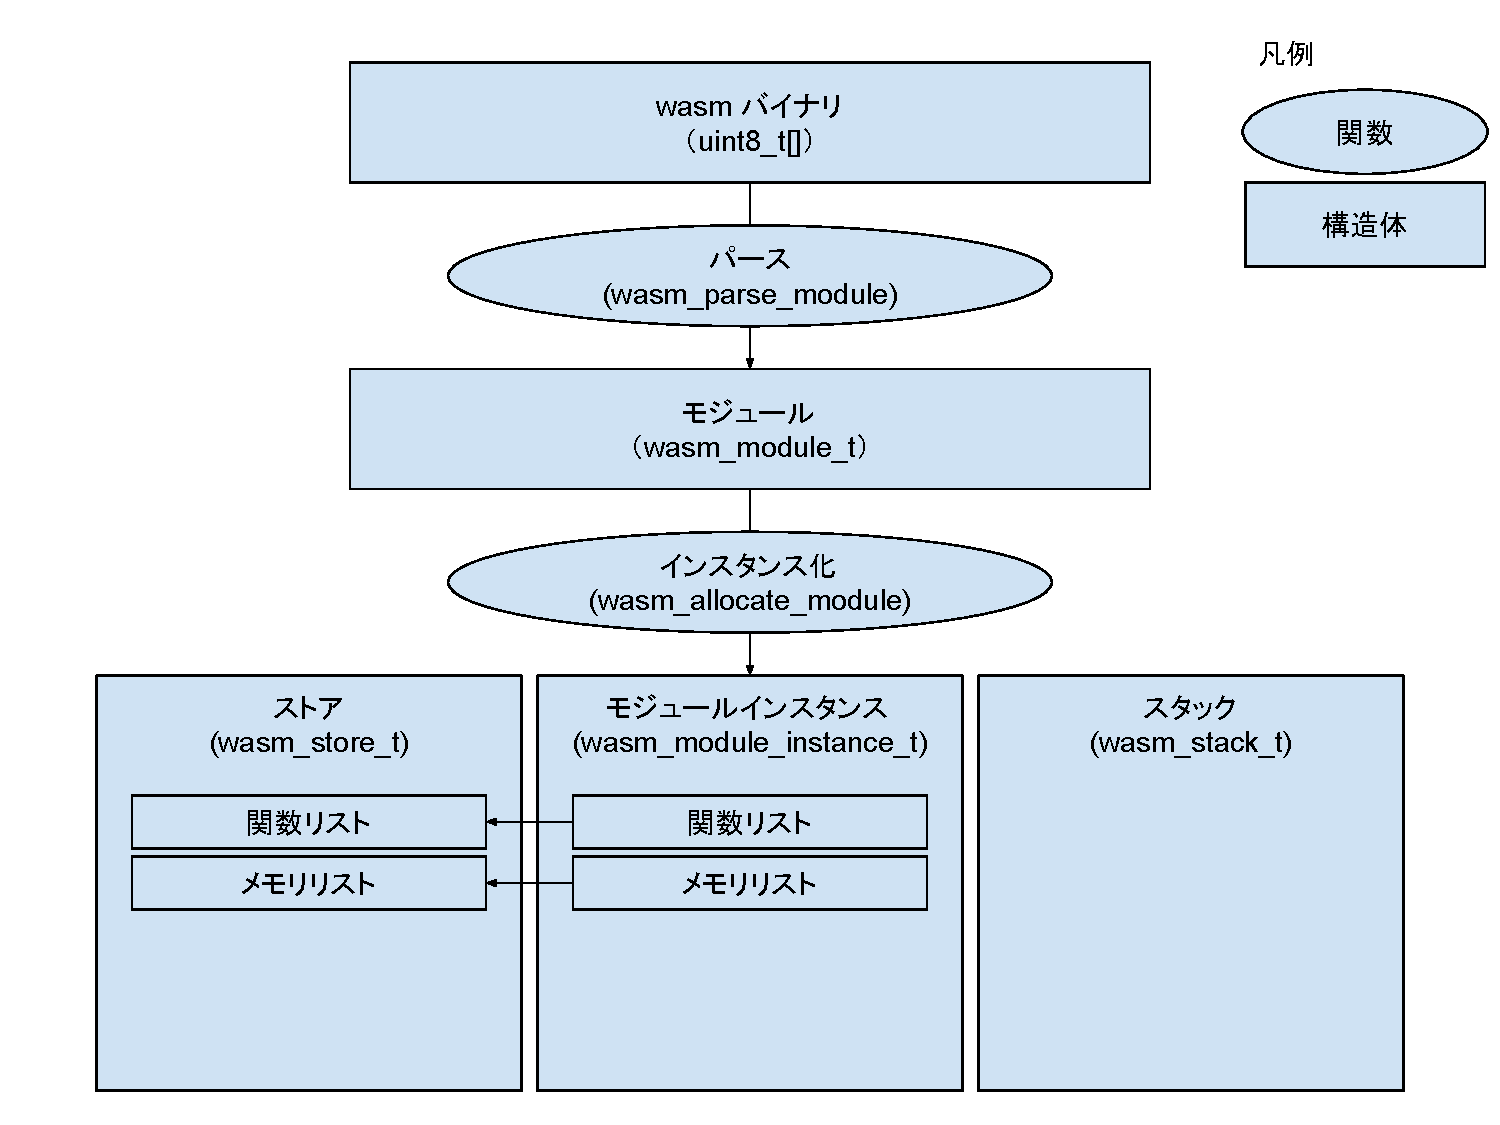
\includegraphics[bb=0 0 800 600,width=12cm]{img/libwasm_arch.pdf}
  \end{center}
\end{figure}
